\documentclass[12pt, onecolumn, conference]{IEEEtran}
%\documentclass[12pt, twocolumn, conference]{IEEEtran}

\usepackage[letterpaper, portrait, margin=1in]{geometry}
\setlength{\parindent}{2em}
\setlength{\parskip}{1em}

\usepackage[]{algorithm2e}
\usepackage{amsmath}
\usepackage{color}
\usepackage{fixltx2e}
\usepackage[pdftex]{graphicx}
\usepackage{listings}
\usepackage[caption=false,font=normalsize,labelfont=sf,textfont=sf]{subfig}
\usepackage{fancyhdr}

\pagestyle{fancy}
\fancyhf{}
\renewcommand{\headrulewidth}{0pt}
\fancyfoot[R]{\thepage}


\definecolor{dkgreen}{rgb}{0,0.4,0}
\definecolor{gray}{rgb}{0.5,0.5,0.5}
\definecolor{mauve}{rgb}{0.58,0,0.82}

\lstset{frame=tb,
  language=Python,
  aboveskip=3mm,
  belowskip=3mm,
  showstringspaces=false,
  columns=flexible,
  basicstyle={\small\ttfamily},
  numbers=none,
  numberstyle=\tiny\color{gray},
  keywordstyle=\color{blue},
  commentstyle=\color{dkgreen},
  stringstyle=\color{mauve},
  breaklines=true,
  breakatwhitespace=true,
  tabsize=3
}

\graphicspath{{../../Images/}}

\begin{document}
 
\title{Crowd Scene Tracking}

\author{\IEEEauthorblockN{Michael Feist}
\IEEEauthorblockA{mdfeist@ualberta.ca}\\
\IEEEauthorblockN{Maciej Ogrocki}
\IEEEauthorblockA{ogrocki@ualberta.ca}
\and
\IEEEauthorblockN{Tamara Bain}
\IEEEauthorblockA{tbain@ualberta.ca}\\
\IEEEauthorblockN{Benjamin Lavin}
\IEEEauthorblockA{blavin@ualberta.ca}}

% make the title area
\maketitle

\begin{abstract}
The goal of this project was to emulate marker motion capture on a large group of people by accurately tracking a crowd of pedestrians and simulating these tracks in a 3D environment. Using only single-camera video data of sparse and dense crowds we combine macro and micro motion capture techniques to detect and track individuals in a crowd. Through a combination of Haar cascade object detection, crowd density analysis, and Lucas Kanade tracking  we are able to determine the tracks of pedestrians in a scene and  generate an output file of track positions per each frame of video. These track positions are then fed into our unity simulation script to generate a approximate simulation of pedestrian movement and positioning in the scene. Our results shows that it is possible to detect individuals in a crowd and approximately simulate real world crowds from a single-camera video recording. 

\end{abstract}

\begin{figure*}[!b]
\centering
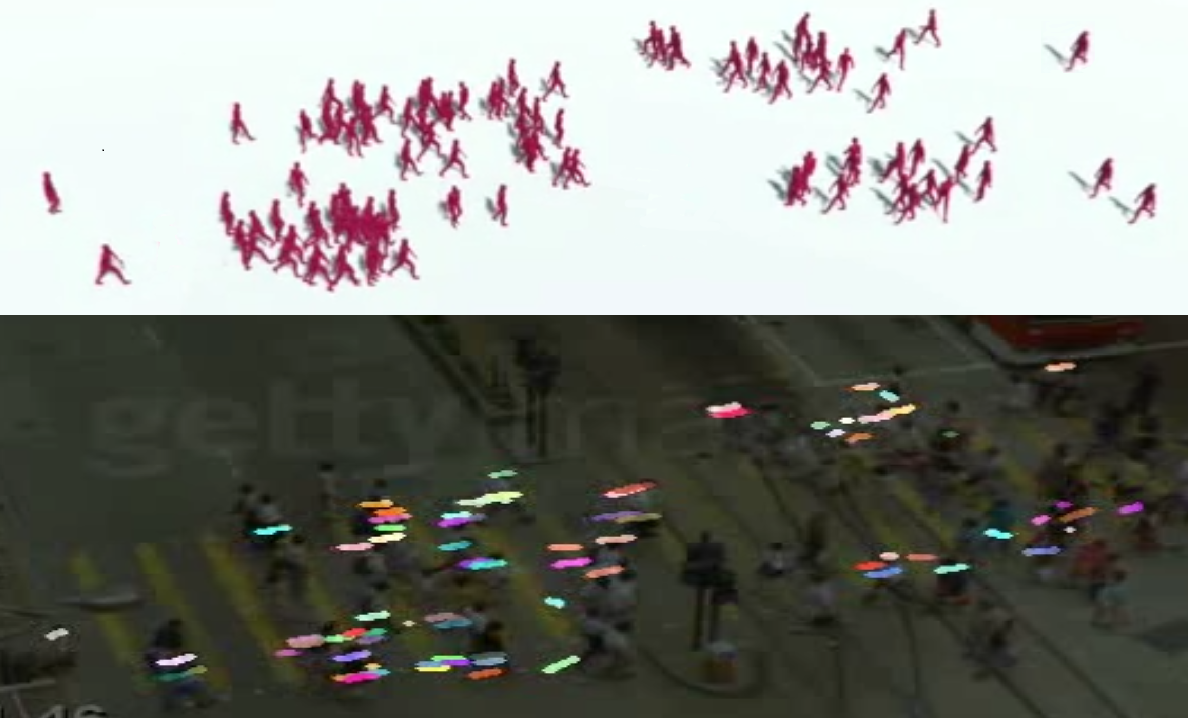
\includegraphics[height=2.5in]{Screenshots/compairsion.png}
\caption{Results of the the completed system showing a simulated crowd and the sample video underneath. }
\label{Compairsion}
\end{figure*}

\section{Introduction}

Automated detection and tracking pedestrians in crowds is a highly studied facet of computer vision, both due to its complexity and its many different applications. The large amount of research has resulted in a diverse range of successful approaches, so that the question of detection and tracking can be answered successfully in more than one way. Approaches can be broken down generally into two sub genres, macroscopic crowd capture solutions, and microscopic crowd capture solutions \cite{A. Yilmaz}\cite{M. Thida}. Macro crowd capture involves looking at the crowd as a whole and utilizes holistic properties of the scene, such as the overall density and flow of moving objects, to determine motion vectors of the crowd \cite{M. Thida}. This approach is popular when simulating crowd scenes for videos or movies, or analyzing the response of crowds to events such as natural disasters. In contrast, microscopic crowd detection and tracking techniques focus on the individual pedestrians within the crowd. Because of the intricacies associated with tracking individuals through a visually cluttered space this method is often more time consuming to implement, but results in more accurate information about the scene and pedestrians at hand. 

Crowd tracking stems from the broader concept of objecting tracking and the difficulties faced are similar to those seen in any object tracking problem. Difficulties can arise due to abrupt object motion, changing appearance patterns of both the object and the scene, nonrigid object structures, object-to-object and object-to-scene occlusions, and camera motion \cite{A. Yilmaz}. These difficulties are more often seen in microscopic crowd tracking techniques because the number of objects being tracked is higher, and the tracked objects are much smaller relative to the scene. 

Both macro and micro crowd tracking solutions have been used in previous literature with varied results. Both techniques have advantages and pitfalls. 

\section{Background}

\subsection{Macro Crowd Capture Techniques}

\subsubsection{Overview of Macro Crowd Capture and Simulation}

Macro crowd capture focuses on gathering information from the crowd as a whole, viewing the crowd as a single fluid entity and relying on data such as: flow, density, scene geography, social forces, and event forces \cite{N. Courty}\cite{B. Boghossian}\cite{R. Mehran}\cite{S. Saxena}. Rather than apply motion capture data to each individual, each individual is classified into a group and is applied a general motion capture file (such as ‘strolling’ or ‘chatting’) \cite{K. Lee}. Macro crowd motion capture has been used to create a realistic crowd that behaves similarly to a real crowd without precise recording of each individual in the crowd. This avoids many of the problems of detection while remaining accurate enough for a wide variety of applications. It has been used to create realistic crowds in movies, video games and other simulations \cite{N. Courty}\cite{R. Mehran}. By detecting specific changes in flow and speed of a crowd it has also been used to computationally detect crowd related emergencies automatically \cite{B. Boghossian}. This can be expanded to detect abnormal behaviours in crowds \cite{S. Saxena}.
Macro crowd motion capture is often a combination high and low-level behavior analysis \cite{K. Lee}. High level behavior analysis looks at information pertaining to the entire crowd such as the flow of the crowd and average speed of the crowd. This type of behaviour has been used to find where a crowd is moving, locations of higher and lower density, and points of entry and exit \cite{N. Courty}\cite{B. Boghossian}\cite{R. Mehran}\cite{M. Rodriguez}.

In contrast, low-level behaviour analysis focuses on groups or individuals within a crowd. This has been used to take data on individual motion, classify it, and apply preset motion capture data based on the classification \cite{K. Lee}\cite{S. Saxena}. 

\subsubsection{High Level Behavior Analysis}

The starting point for high level analysis is flow and speed of the crowd \cite{N. Courty}\cite{B. Boghossian}\cite{R. Mehran}. N. Courty et al., B Boghossian et al., and R.Mehran et al. all used variations on the optic flow algorithm to detect directions of movement in a crowd and use this as a starting point for further analysis and simulation generation. R. Mehran et al. supplemented the optic flow algorithm by applying the social force model to improve their crowd simulation \cite{R. Mehran}. Social force can be described as the behaviour of the crowd as a result of the actions of individuals \cite{R. Mehran}. By computing social force, R. Mehran et al. were able to determine the ongoing behavior of the crowd and its movement towards a goal or destination \cite{R. Mehran}. 
One high level approach for tracking in high density crowds is to use a scene structure based force model\cite{S. Ali}. S. Ali and M. Shah used describe their ‘scene structure force model’ by proposing that individuals moving about a scene are subject to local and global forces that influence the individual’s locomotive behaviour. Three floor fields are described which determine the individual’s probability of movement from one location to another \cite{S. Ali}. The Static Floor Field (SFF) is the attraction field. This represents the typical crowd motion toward attractive locations in the environment, for example, the exit door. The Boundary Floor Field (BFF) represents the repulsive forces that shape the motion paths of crowds such as fences, walls, or other obstacles. Finally, the Dynamic Floor Field (DFF) is representative of the immediate behaviour of other sections of the crowd in the vicinity of the specific section being analysed. The collective behavioural patterns represented by these fields can be combined then constrain the likely locations or paths that can be taken by the target in the scene \cite{S. Ali}. 
An analysis of high level behavior has been shown to be sufficient for detecting abnormalities in crowds \cite{R. Mehran}\cite{F. Zhao}. However such analysis falls short of pointing out what the abnormal behavior or actions actually look like, such detail requires a low-level analysis of the crowd behavior.

\subsubsection{Low Level Behavior Analysis}

Several types of low level behavior analysis have been used to increase detail in crowd simulations resulting from macro motion capture \cite{K. Lee}. K. Lee et al. looked at individuals in a crowd and classifies them by the type of action they were performing. By applying preset motion capture data based on these classifications, the detail in the resultant crowd simulation was improved \cite{K. Lee}. 
Using this system it was possible to have simulated individuals perform specific actions such as dancing and cheering \cite{K. Lee}. As opposed to the high level behaviour studies in which the individuals only simply walk \cite{N. Courty}\cite{R. Mehran}.
A major issue with low level behaviour is that it uses pre recorded motions that are then applied to a models using the information gathered from the input video. By doing this multiple individuals will perform the same actions causing a clone effect \cite{R. McDonnell}. The most optimal way to fix this is to have many pre recorded motions; this however, is expensive. R. McDonnell et al. use proximity and model typing to create heterogeneous crowds without having to increase the amount of animations \cite{R. McDonnell}.
The algorithm described in S. Saxena et al. used KLT (Kanade-Lucas-Tomasi) to track feature points. Using KLT is handy because it automatically gives the 2-dimensional motion vector for each feature point. After tracking the feature points, the next step is to clean up the data. To clean up the data, first feature points that remain stationary are removed as these points are most likely due to noise or belong to background objects. Next, points that are relatively similar in location and direction are clustered together.
The method in S. Saxena et al. tracks the crowd’s principal direction, speed, and mobility. Direction is calculated by using a histogram of all the motion vectors for a cluster. A histogram is used in order to determine if a crowd is showing abnormal behavior; this occurs when the cluster has multiple directions. Speed is measured by analysing the change in the location of the crowd. For this approach to work, the camera needs to be calibrated. The calibration involves the use of “two pairs of parallel lines (perpendicular to each other) on the ground and the height of a reference object” \cite{S. Saxena}. The authors do not go into detail of how mobility is calculated, but they seem to simply track the change in the number of feature points for each cluster. “This attribute can thus be used to determine abnormal events if the number of valid feature points changes drastically” \cite{S. Saxena}.
A.B. Chan et al. proposed a method that is able to track individuals without using  object/pedestrian detection or feature tracking. First the scene is segmented into crowds with different motions \cite{A.B. Chan}. Next features are extracted from each crowd segment. Finally, the number of people per segment is estimated with Gaussian process regression.

\subsubsection{Limitations}

High level behaviour can be used to detect the flow and behaviour of a crowd but will lack the specific details that can be found in tracking and capturing the actions and movement of each individual. R. Mehran et al. demonstrated simulated crowds moving in a realistic approximation of a crowd but are unable to directly capture information of a real world crowd and simulate it \cite{R. Mehran}. 
In fields such as risk assessment or emergency procedure evaluation, where individual actions are valuable, a more detailed analysis than can be afforded by macro crowd capture should be used.
One downfall to the method proposed in cacro crowd capture is that it groups people together as opposed to tracking each individual person. This approach makes it difficult to determine crowd density. R. Mehran et al. do not seem to address this issue, but they do explain previous work in the field that has solutions to crowd density \cite{N. Courty}\cite{R. Mehran}\cite{S. Saxena}. 
The algorithm proposed by A.B. Chan et al. has the ability to give us an accurate density of the crowd. However, the method requires that training be run on a subset of the data. In the paper, the authors described how they first trained on 800 frames and then ran the testing on 1200 frames \cite{A.B. Chan}. Because of the need for training, one could not simply grab utilize a feed from any camera source and expect the algorithm to work instantaneously. Instead, the user must manually train the method to estimate the density, a very time consuming process.

\subsection{Micro Crowd Capture Techniques}

\subsubsection{Overview of Micro Crowd Capture}

In contrast to the macro techniques described above, micro crowd motion capture eschews simulation of a crowd for detection and tracking of distinct individuals. Many studies follow a similar basic algorithm in this regard, starting with object detection of pedestrians, and following with some method of object tracking \cite{M. Rodriguez}\cite{D. Zhang}\cite{I. Ali}\cite{F. Zhao}\cite{I. Ali2}. The major challenges of micro crowd capture are occlusion, adequate detection, false positives, and perspective. Most studies attempt to supplement their detection and tracking with some additional algorithm or technique to address challenges such as occlusion, false positives, and varying camera perspective. 
Despite the highly successful nature of many of these studies, they are still limited by large training sets, and may be situational applicable depending on the density of the crowd or the number of cameras used.

\subsubsection{Object Detection}

Pedestrian-detection is often the first step in micro crowd capture techniques. In dense crowds two hurdles for accurate detection are large areas of occlusion and varying perspectives of moving objects. Many studies address occlusion of pedestrian bodies by focussing on head detection \cite{M. Rodriguez}\cite{D. Zhang}\cite{I. Ali}\cite{I. Ali2}. The Viola and Jones Haar-like AdaBoost cascade detector is cited frequently as the preferred method of object detection and is trained to classify pedestrian heads \cite{D. Zhang}\cite{I. Ali}\cite{I. Ali2}. Using this method requires large training sets of images (4000+) as well as half as many negative images. The large size of the training set is partially due to the multiple potential perspectives of the human head as a pedestrian moves throughout the scene. Each potential perspective and distortion of a human head must be trained for to ensure high detection rates. As an alternative to the Viola and Jones detector and to address these potential variations in viewpoint, Rodriguez et al. utilizes a parts based model which has improved detection accuracy on deformed datasets \cite{D. Forsyth}.
Object detection is a balance between adequate detection and the reduction of false positives. After settling on an adequate detection method many studies apply a secondary measures to reduce false positives such as scene geometry, energy expenditure, or crowd density \cite{M. Rodriguez}\cite{D. Zhang}\cite{I. Ali}\cite{I. Ali2}. Scene geometry is an easy way to improve detection results. By noting the average position of heads within a scene, and knowing the average size of a human head, the position of the ‘Head Plane’ can be calculated. Using a head plane and calculating the expected size for each head within that plane makes it possible to take depth into account in single camera scene captures \cite{M. Rodriguez}\cite{I. Ali2}.  Other studies use scene geometry to surmise most-likely paths of motion in a scene \cite{M. Rodriguez}\cite{D. Zhang}.  D.Zhang et al. favors detection of objects occurring along likely scene trajectories \cite{D. Zhang}. 
These enhancements to object detection can be applied in succession to refine results. M. Rodriguez et al. uses both scene geometry and crowd density to reduce false positives and improve head detection in crowds. Their detection rate and number of false positives are better when both methods are used \cite{M. Rodriguez}. 

\subsubsection{Single Camera Tracking}

Occlusion is one of the major problems when tracking individuals with single cameras in high density scenes. The method proposed by V.K. Singh et al. tries to solve this issue \cite{V.K. Singh}. The tracking problem is divided into two stages. In the first stage, a tracking algorithm tracks individuals and, if it briefly loses track of an individual, simply tracks the reappearance as a new individual. In the second stage, the algorithm attempts to combine multiple motions together which belong to the same individual.
D. Zhang et al. manage occlusion during tracking by devising a set of heuristics for favoring energy conservation within a scene. These heuristics filter out trajectories that would place two pedestrians on the same path at the same time, have pedestrians appear suddenly in the middle of the scene or have pedestrians greatly vary their speed/position within a short period of time \cite{D. Zhang}. This method improves the robustness of tracked trajectories over multiple iterations.

\subsubsection{Multi Camera Tracking}

An idea proposed to help track dense crowds and handle occlusion is to use multiple cameras that overlap the scene instead of a single camera \cite{R. Eshel}\cite{M. Liem}. R. Eshel and Y. Moses used multiple cameras and were able to detect a person's head without using any object detection\cite{R. Eshel}. This is achieved by applying a homography to map all the cameras to a unique plane that is parallel to the ground and at the height of the person's head. This means the same point on the plane will map to the same image location in all cameras. If an object does not fall on the plane then it will not align in the multiple views after the homography is applied. Because of this they are able to isolate the head by looking at what moving objects align on the plane. Once the head is tracked, the speed and direction can be estimated using the previous frame \cite{R. Eshel}. If the head being tracked does not move relatively in the same motion, then it is treated as a false positive and discarded. The issue with their method is that their algorithm assumes a "set of synchronized and partially calibrated cameras overlooking a single scene, where head tops are visible." 

Finally, it is important to note that the results improve as more cameras are added \cite{R. Eshel}. Better results are seen once 5 cameras have been added, however once the number of cameras reaches 7, the benefits of adding further cameras are negligible.
M. Liem and D. Gavrila’s method is similar to R. Eshel and Y. Moses’s algorithm. Both algorithms try to recreate a 3D environment \cite{R. Eshel}\cite{M. Liem}. However, M. Liem and D. Gavrila’s method first uses volume segmentation to try and separate a person, followed by a combination of feature points and likelihood functions to predict which volumes are individual people \cite{M. Liem}.


\subsection{Combining Micro and Macro Crowd Capture}

Several studies combine macro and crowd capture to refine their results. Rodriguez et. al use macro analysis of crowd density to improve head detection and tracking of individual pedestrians \cite{M. Rodriguez}. In contrast F. Zhao et. al use micro analysis of a pedestrian scene to supplement a macro style detection of abnormal activity \cite{D. Zhang}. Studies like these show that micro and macro crowd capture are not mutually exclusive and can be used in tandem to improve the accuracy of results. 

\section{Implementation}

\subsection{Density}

\begin{figure*}[!t]
\centering
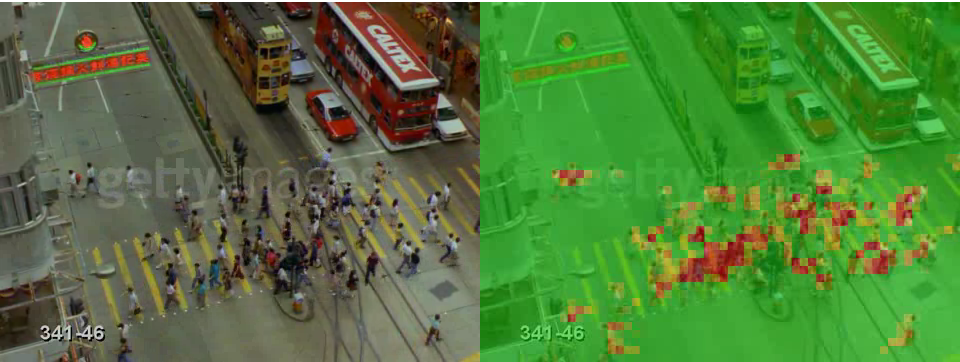
\includegraphics[height=2.5in]{Screenshots/Density.png}

\includegraphics[height=1.8in]{Screenshots/Capture15.png}
\caption{Results of the density algorithm. Green for areas with low density, yellow for areas of medium density, and red for areas of high density.}
\label{Density}
\end{figure*}

One parameter of the crowd that was useful in other areas of the project was crowd density. In order to calculate the density of a crowd we need to make some assumptions. The first is that the people in the crowd are all moving roughly the same speed. Next we have to assume that the size of a person stays roughly the same as they move through the scene. Finally we assume that the more an area in the scene is changing the more people are in that area.

With these assumptions we are able to calculate the density of a crowd by calculating the temporal difference. To calculate the temporal difference we simply take the current frame and subtract it from the previous frame. We then take the difference and create a threshold image. We found that a change in magnitude greater than 20 was significant enough to warrant valid change. We did not want to include all changes in the threshold image since then the threshold would include noise from the camera. Next we divide the scene into smaller blocks. For scenes like the ones shown in Fig. \ref{Density} we found block sizes of 8 by 8 worked well. Next we iterate over the blocks and calculate the percentage of change. We then add the percent of change multiplied by some growth rate to the density map. Also it is important to decrease the density of the blocks over time.

\begin{algorithm}
\DontPrintSemicolon
 $I_{t} \leftarrow | Im[x, y, t+1] + Im[x, y, t] | $\;
 $I_{threshold} \leftarrow I_{t} > threshold$\;
 $blocks_{x} = Im_{width}/block_{size}$\;
 $blocks_{y} = Im_{height}/block_{size}$\;
 \For{i := 0; i $< blocks_{x}$; i++}{
  \For{j := 0; j $< blocks_{y}$; j++}{
   $density[i, j] \leftarrow I_{density}[i, j]  - decay \  rate$\;
   \If{$density[i, j] < 0$} {
    $density[i, j] \leftarrow 0$\;
   }
   $x1 \leftarrow i(block_{size})$\;
   $x2 \leftarrow i(block_{size}) + block_{size}$\;
   $y1 \leftarrow j(block_{size})$\;
   $y2 \leftarrow j(block_{size}) + block_{size}$\;
   $block \leftarrow I_{threshold}[x1:x2, y1:y2]$\;
   $density[i, j] \leftarrow density[i, j] + \alpha\sum_{x}^{N} \sum_{y}^{N} block [x, y]$\;
   \If{$density[i, j] > 1$} {
    $density[i, j] \leftarrow 1$\;
   }
  }
 }
\caption{Density Calculation}
\end{algorithm}

\subsection{Optic Flow}

Optic Flow has been discussed in the literature as a way to calculate the flow of the crowd \cite{N. Courty}\cite{B. Boghossian}\cite{R. Mehran}. Most of the research used the calculated flow information in a simulator. However, since we did not have a simulator the flow information of the crowd was not as useful to us. That being said we still were easily able to calculate the flow of the crowd using OpenCV’s built-in Optic Flow function. \\

\begin{lstlisting}
flow = cv2.calcOpticalFlowFarneback(prev_gray, gray, None, 0.5, 3, 20, 3, 5, 1.2, 0)
\end{lstlisting}

There are a few issues with using Optic Flow to calculate the flow of the crowd. The first is that when two objects are moving against each other they will cancel out the flow of both objects. Second, flow is not calculated equally over all objects in the crowd. Larger objects will have a greater impact on the flow of the crowd as they will take up more space and appear as multiple pedestrians. Videos that contain large non-pedestrian objects such as cars will be less accurate.

\begin{figure*}[!t]
\centering
\subfloat{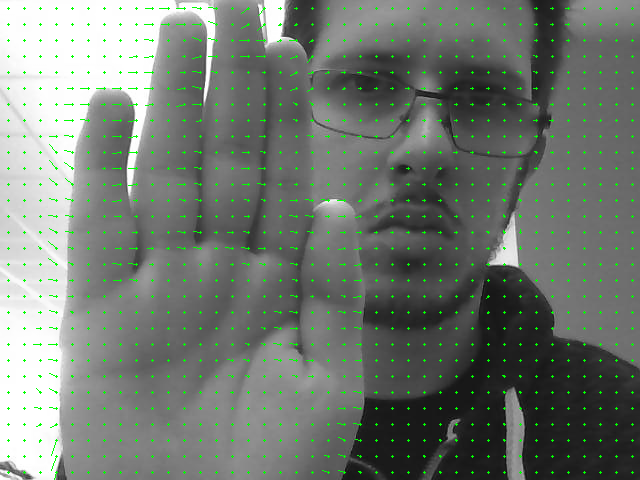
\includegraphics[width=2.5in]{Screenshots/OpticFlow_image_72.png}%
\label{OF_first_case}}
\hfil
\subfloat{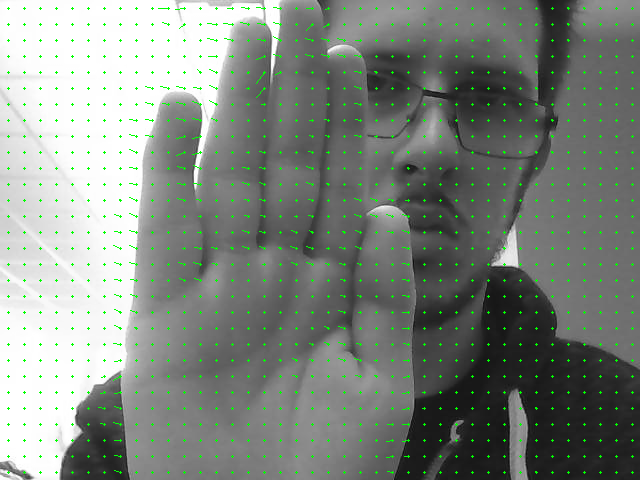
\includegraphics[width=2.5in]{Screenshots/OpticFlow_image_79.png}%
\label{OF_second_case}}
\caption{Results of the Optic Flow algorithm. Small lines point in the direction in which the pixels are found to be moving. In this image you can see that the hand is moving very slightly from left to right.}
\label{Optic_Flow}
\end{figure*}

\subsection{Affine and Metric Rectification}

Most video feeds are not placed above the scene and angled orthogonal to the ground plane. In other words the video feed is not always at a perfect bird's eye view of the scene. Because of this, the information calculated is skewed with distance. The farther away an object is from the camera the less an object will appear to move. This concept can be illustrated if one was to take an image of a meter stick from a close distance and then one from far away. When meter stick  placed farther away from the camera, it will appear smaller in the image.

\begin{figure*}[!t]
\centering
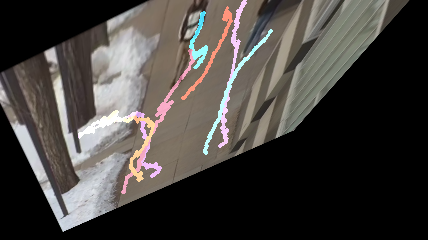
\includegraphics[height=2.5in]{Screenshots/HaarCascade_HomographyAppliedTracks.png}
\caption{Recorded tracks after a metric rectification was applied.}
\label{Rectification}
\end{figure*}


We can attempt to remove the projective distortion and fake a top-down view of the scene by applying a metric rectification. Following the solution proposed in section 2.7 of Hartley and Zisserman's book, Multiple View Geometry, we were able to implement a two pass metric rectification algorithm. The first step is the user selects two pairs of parallel lines. Using these lines we are able to apply an affine rectification using the following equations.

\begin{equation}
v_1 = m \times m'
\end{equation}

\begin{equation}
v_2 = n \times n'
\end{equation}

\begin{equation}
l = v_1 \times v_2
\end{equation}

\begin{equation}
H =
\begin{bmatrix}
1 & 0 & 0\\ 
0 & 1 & 0\\ 
l_1 & l_2 & l_3 
\end{bmatrix}
\end{equation}

Where m and m` are one set of parallel lines and n  and n` are the other set of parallel lines.

Next we have the user select two pairs of orthogonal lines in the affine rectified image. Using the orthogonal lines we are able to retrieve a metric rectified image from the affine image. Finally we allow the user to scale, rotate, and translate the results to allow them to get a better viewing experience. When the user is happy with the results they can output the matrix to the screen allowing them to use the homography matrix in the tracking algorithms described below.

\subsection{Tracking With Lucas-Kanade}

\begin{figure*}[!t]
\centering
\subfloat{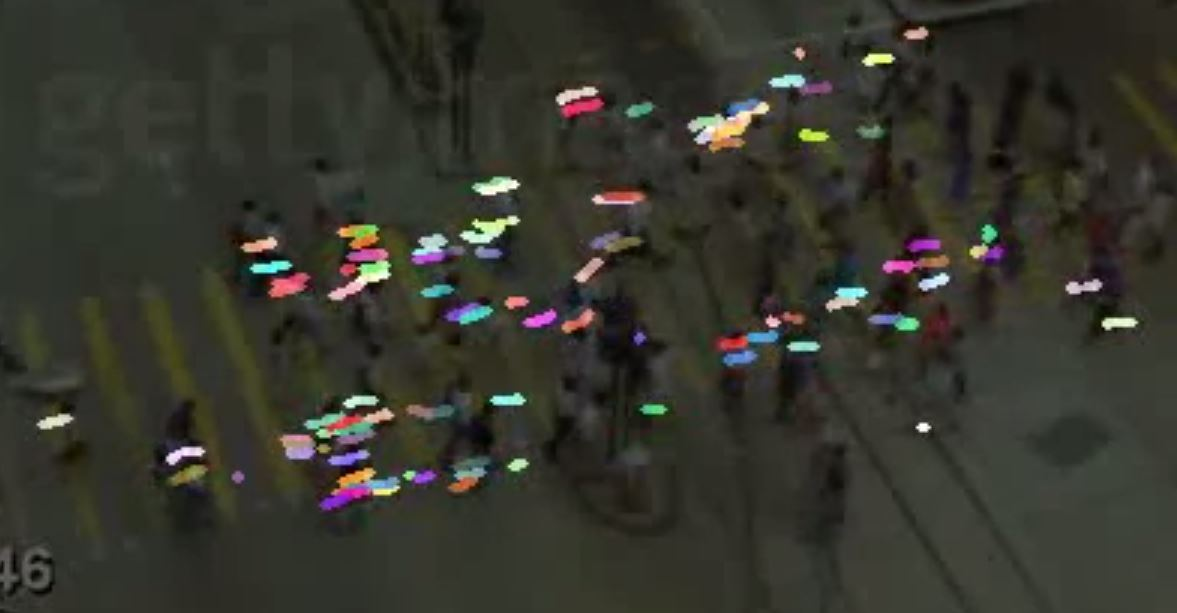
\includegraphics[width=3.5in]{Screenshots/Capture1.JPG}%
\label{LK_first_case}}
\hfil
\subfloat{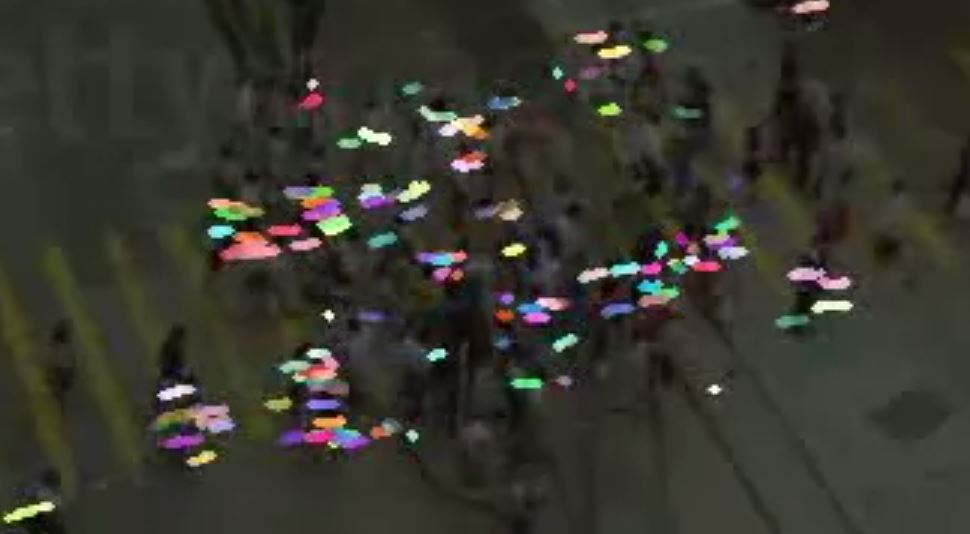
\includegraphics[width=3.5in]{Screenshots/Capture2.JPG}%
\label{LK_second_case}}
\caption{Results of the Lucas-Kanade tracking algorithm.}
\label{LK Tracking}
\end{figure*}

One technique used to track people in a crowd was an implementation of Lucas-Kanade that tracked feature points. We begin by searching through the first frame in the video feed to find feature points. These feature points are areas in the image where corners are found. More specifically we used Shi-Tomasi corner detection. After we have our points we create a new track for each point.

We then start the main loop of the tracking algorithm. The loop starts by grabbing the next frame in the video feed and then trying to find the new locations of the feature points with help from Optic Flow. OpenCV has a nice built-in function that takes the points from the previous frame, p0, and tries to calculate the points' current location, p1.

\begin{lstlisting}
# The variable ‘p0’ is the original location of the points and ‘p1’ is the new location
p1, st, err = cv2.calcOpticalFlowPyrLK(prevgray, gray, p0, None, **lk_params)
\end{lstlisting}

Since people can move in and out of the frame we added a section of code that would add new feature points to the scene. This works by first finding areas of change between the current frame and the previous frame. Next we search for new feature points in these areas of change. Finally we add the new feature point to our tracking points if that new feature point does not have a similar corresponding tracking point. These are points in relatively the same location.

We also try to remove points from the list of feature points, p1, that are no longer valid. The points that are removed are points that no longer move or move an unrealistic amount. The main issue with removing points that remain still for an extended period of time is that we can easily remove points that belong to a person that has briefly stopped moving and will continue moving. Because of this we need to assume that people are not stopping for this algorithm to work correctly.

\begin{center}
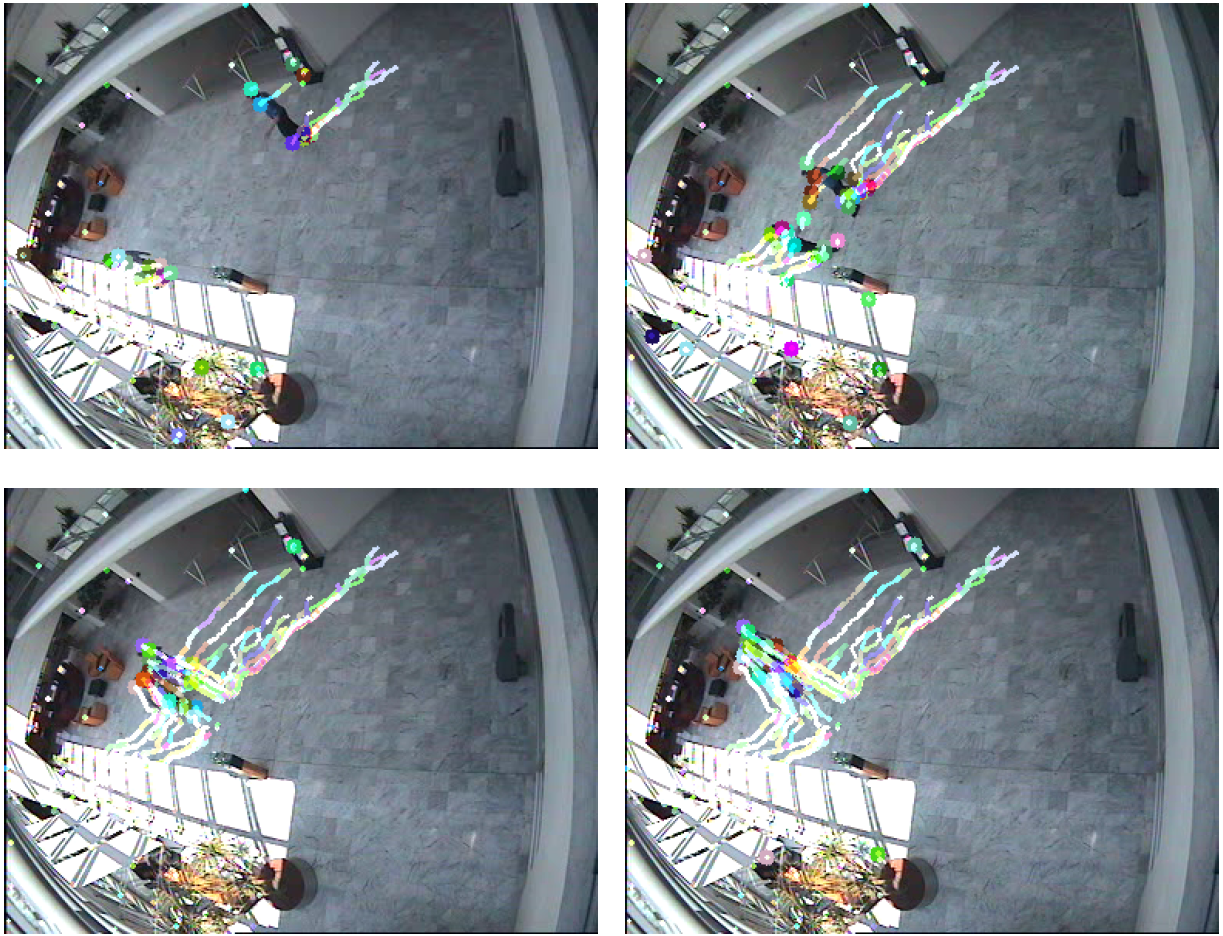
\includegraphics[height=3.5in]{Screenshots/Capture12.PNG}
\end{center}

After we have our updated list of feature points, p1, we need to add the points to their corresponding track. This posed some initial difficulties since the size of p1 is constantly changing and the indexed points do not always correspond to the same indexed track. In order to store and update all the changing information we have four arrays.

\begin{enumerate}
\item p1: An array of all the active points. These are the points currently being tracked by Lucas-Kanade.
\item st: An array of which points in p1 are no longer active and were removed from p1 during this last iteration. It is a bit array where 1 means that the point is still active and 0 means that the point was deleted.
\item tracks: A 2D array storing the path that each point tracks. It is an m x n array where m is the number of frames and n is the number of points.
\item tracks\_index: Since p1 and tracks do not match in size or indexing, we need tracks\_index to keep a map between p1 and tracks.
\end{enumerate}

The tracks\_index array is first initialized with values 0 to n-1, where n is the number of points in p1. With each iteration we obtain a list of the points which were deleted from p1, st. We then iterate over st and, if a point is removed, we set the value in tracks\_index corresponding to the index in st to -1, and subtract one from all the remaining values in tracks\_index. This can be seen in Table \ref{table_index}.

\begin{table}[!t]
\caption{A simple example of how track\_index is updated}
\label{table_index}
\centering
\begin{tabular}{ | l | c | r | }
 \hline
 Array & Values\\
  \hline                 
  $st$ & $[1, 1, 1, 0, 1, 1]$\\
  $tracks\_index\ before\ update$ & $[0, 1, 2, 3, 4, 5]$ \\
  $tracks\_index\ after\ update$ & $[0, 1, 2, -1, 3, 4]$ \\
  \hline  
\end{tabular}
\end{table}

After this step, if p1 has more points than the max value in tracks\_index, it means that an additional point was added. In this case we append the max value plus one to the end of tracks\_index. This can be seen in Table \ref{table_index_add}.

\begin{table}[!t]
\caption{A simple example of how elements are added to track\_index}
\label{table_index_add}
\centering
\begin{tabular}{ | l | c | r | }
 \hline
 Array & Values\\
  \hline           
  $tracks\_index\ before\ update$ & $[0, 1, 2, -1, 3, 4]$ \\
  $tracks\_index\ after\ update$ & $[0, 1, 2, -1, 3, 4, 5]$ \\
  \hline  
\end{tabular}
\end{table}

Finally we go through p1 and find where the index of the current point in p1 is located in tracks\_index. Given where the point in p1 was found in tracks\_index we then add the point in p1 to the correct path in tracks.

After we have finished recording all the tracks we do a couple passes to clean up the data before we output it to a file. For example we delete tracks that we deem to short and were probably just some random blip. We also remove tracks that do not seem to follow a consistent path.

\subsection{Object Detection}

In the literature the most commonly used detectors for pedestrians are head detectors, upper body detectors, and full body detectors \cite{G. Shu}\cite{P. Viola}. OpenCV has haar cascade classifiers for pedestrian upper-body and full-body available in their github repository\cite{Itseez}. However upon testing we found that these pre-existing classifiers offered poor detection on dense crowds and only offered detection from the front and back views. As a result we decided to train our own Haar cascade classifier following the steps outlined in Naotoshi Seo’s OpenCV haartraining tutorial \cite{N. Seo}. 

The first step of Haar detection is gathering images for the classifier training set. Lienhart et. al. recommends at least 5000 positive and 3000 negative images, with larger datasets increasing the chance of detection and reducing the number of false positives detected \cite{R. Lienhart 1}. A dataset consisting of crops of pedestrian heads would be ideal for detection in dense crowds. Unfortunately no such dataset was available to us. Instead we settled for the INRIA Person Dataset which was originally used for a histogram of gradients human detection algorithm \cite{INRIA}\cite{N. Dalal}. This dataset consists of  16734 cropped images of standing and walking pedestrians viewed from the front, side and behind and 1672 non-pedestrian images for use as negatives. We used ImageMagick’s `identify` command to output the coordinates of the bounding box for each cropped pedestrian image to a data file. This data file was then passed to OpenCV’s createsamples utility to generate the appropriate vec format file. Our set of positives was large enough that no additional transformations or color modifications were needed to generate additional positives. 

This process was repeated a second time with a smaller subset of INRIA positives consisting of only 5000 images of pedestrians. This smaller dataset was used initially for haar training in order to estimate the time required to train the larger 16000 positive dataset. Training was completed using OpenCV’s traincascade utility. Following the work of Viola and Jones we trained with 20 cascade stages \cite{P. Viola}. More cascade stages increases the precision of the cascade, but too many cascade stages risks overtraining the cascade and prevents the acceptance of objects that would otherwise be recognized as matches. We also utilized the extended version of the Haar feature set, which includes 45 degree rotations of the original feature set \cite{R. Lienhart 2}. Training took 47 hours using a 8-core Intel 3.4GHz i7-2600K CPU with multi-threading enabled. For the larger dataset of 16000 positives, training took 107 hours. 

The resulting cascade XML files were loaded into OpenCV. The cascade classifier required manually tuning for each test video. The 5000 positive classifier was significantly out performed by the 16000 positive classifier on all videos. 

\begin{figure*}[!t]
\centering
\centering
\subfloat{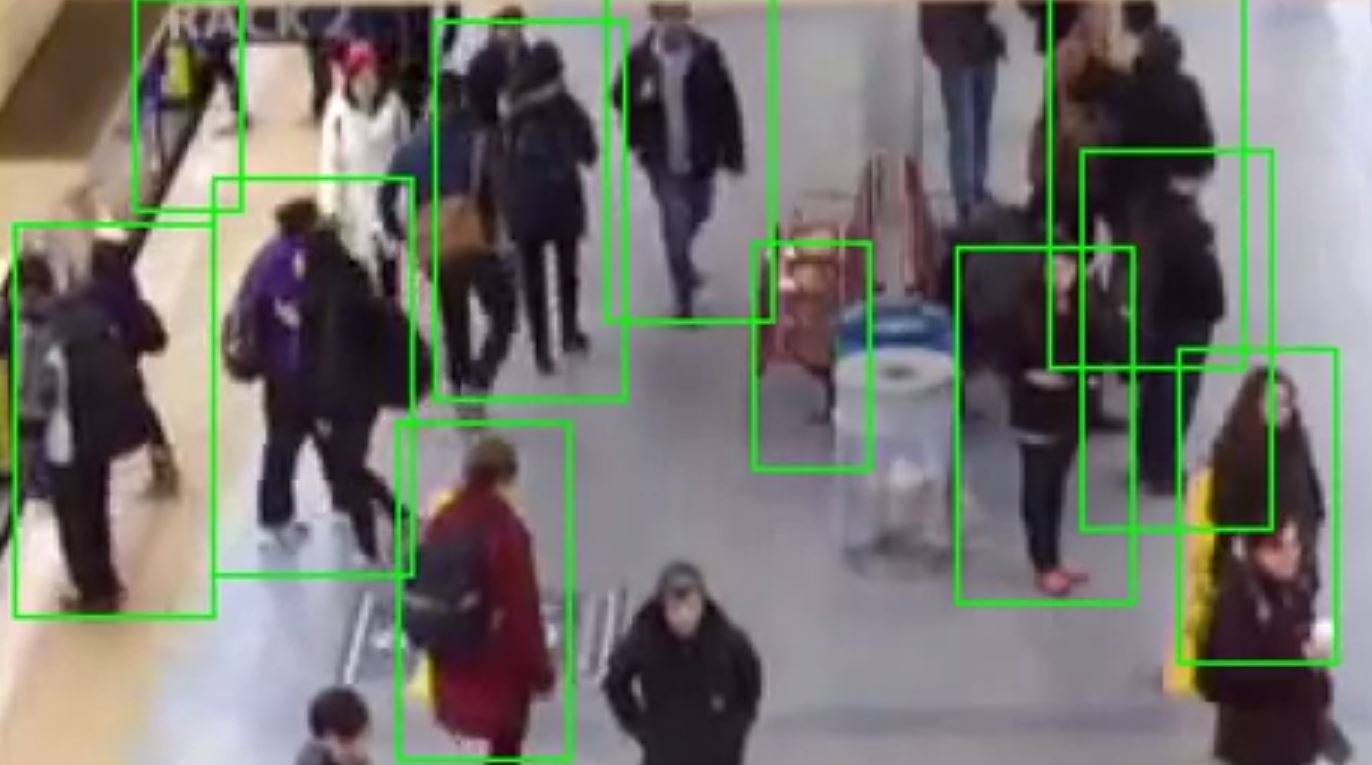
\includegraphics[width=2.5in]{Screenshots/Capture5.JPG}%
\label{OB_first_case}}
\hfil
\subfloat{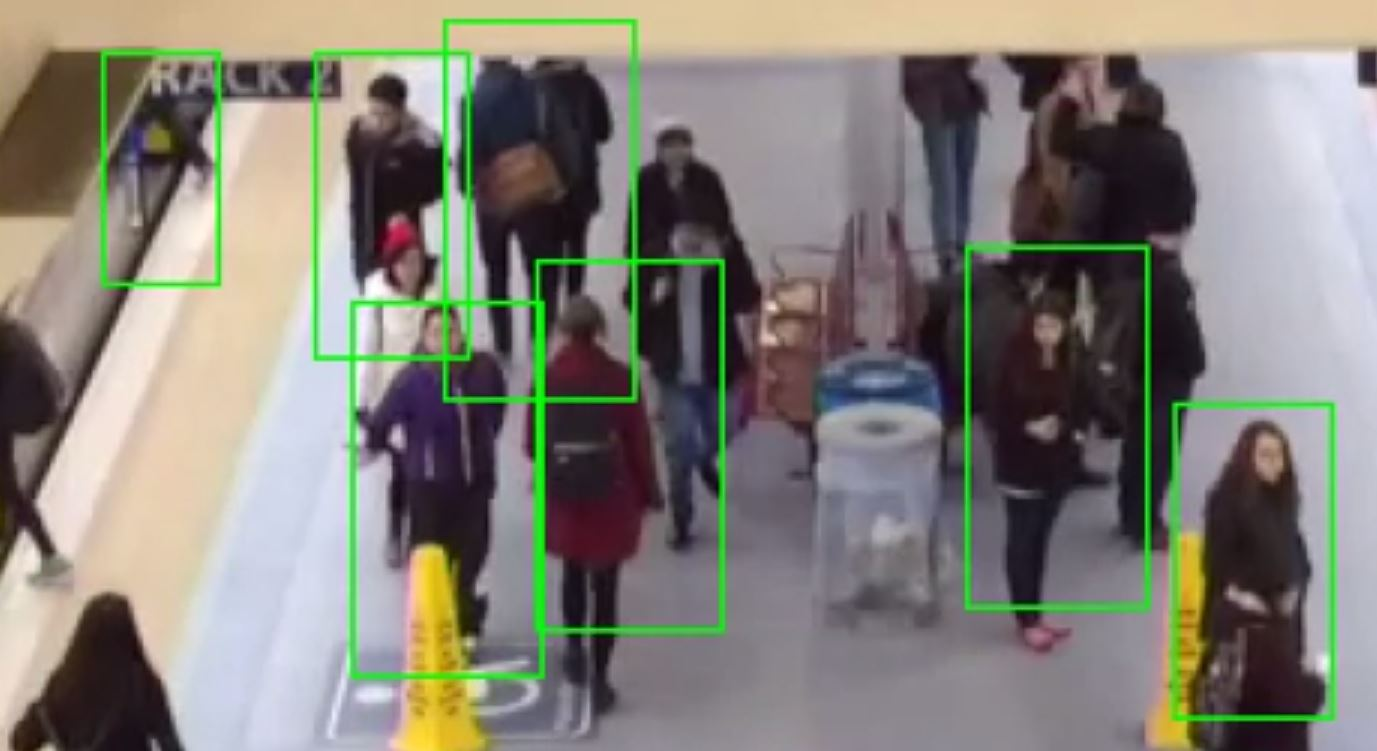
\includegraphics[width=2.5in]{Screenshots/Capture6.JPG}%
\label{OB_second_case}}
\caption{Results of our trained Haar cascade pedestrian detector. Video captured from the University of Alberta LRT station.}
\label{Object_Detection}
\end{figure*}

\subsection{Tracking with Object Detection}

\begin{figure*}[!t]
\centering
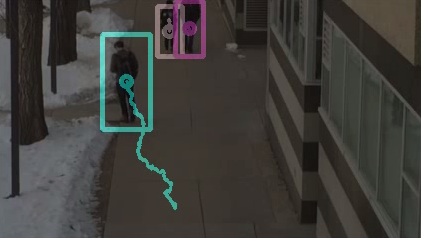
\includegraphics[height=2.5in]{Screenshots/OB_Tracking.png}
\caption{Results of the tracking algorithm that utilizes the Object Detection.}
\label{Tracking_Object_Detection}
\end{figure*}

We were able to implement a tracking algorithm that utilizes the object detection described above. For each frame in the video we first run the object detection over the scene to find possible people to track. The object detection on its own gives us some false positives. In order to remove some of these false positives we combined the object detection with our density calculation. Now if a detected object is in an area of low density it is removed as there is most likely no one there. The main issue with this approach is we miss people who are standing still for an extended period of time. We can still handle the case when a person just briefly stops.

After we have our detected objects we try to find where these objects were in the last frame. For each detected object we compare the distance between the current object and the objects detected in the previous frame. If the distance is over a threshold we deem that the two detected objects do not belong to the same person. In the case when multiple objects from the current frame are possible matches to the same object in the previous frame, we simply pick the pair with the smallest distance.

We also store the path these objects take which we refer to as a track. After we have matched all the detected objects with the objects in the previous frame we are able to add each individual object to the correct track. If an object does not have a match then we deem it a new object and create a new track. However, if a track has no new objects added to it in the last n frames, where n is some number that the user decides is appropriate for the video, then the track is ended and the track can no longer be updated with new object locations. If a track is ended and is less than some threshold of frames then we remove the track as it is deemed an error.

\subsection{Output}

Using the information that we gathered from the above tracking methods we are able to create a output file with the track information. This output file is formatted into two sections.

The first section lists pairs of integers, with each pair representing a single track. The first integer states the starting frame (the frame in which the track first appears), and the second integer provides the number of frames for which the track appears. 

The second section of the output file contains pairs of floats representing X and Z coordinates in a 3D environment. The pairs are listed in the same order that their respective tracks appear in the first section, and contain the coordinates for each frame of the tracks. An example output file is shown in Fig. \ref{Output}.

\begin{figure}
\begin{gather*}
0\ 220 \\
0\ 244 \\
...  \\
233\ 12 \\
236\ 9   \\
 \\
379\ 252 \\
377\ 251 \\
...  \\
348\ 147 \\
356\ 146 \\
\end{gather*}
\caption{Example output file. It shows that track 1 first appears at frame 0 and goes for 220 frames. Then track 2 appears at frame 0 as well but goes for 244 frames. The coordinates for each track begin after the new line in the middle of the file. The first frame in track 1 is at position (379, 252) and the second frame is at (377, 251).}
\label{Output}
\end{figure}

\subsection{Unity}

\begin{figure*}[!t]
\centering
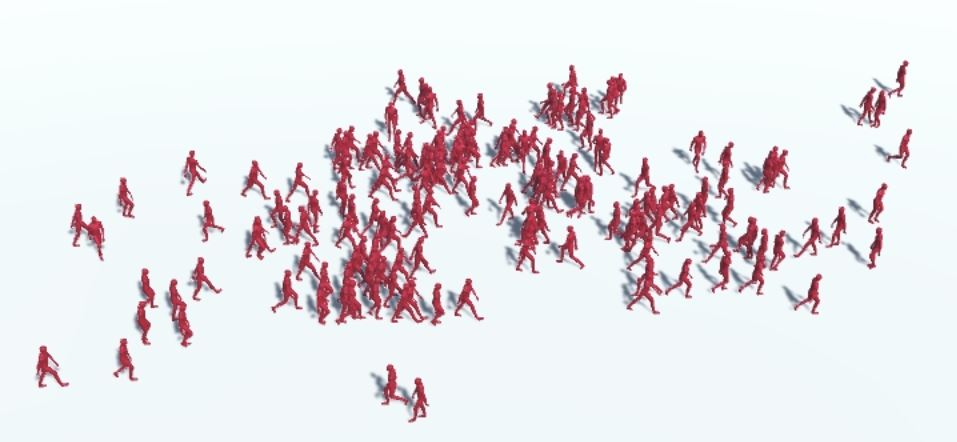
\includegraphics[height=2.5in]{Screenshots/Capture4.JPG}
\caption{Results of the Unity crowd playback data outputted from the tracking algorithms.}
\label{Unity}
\end{figure*}

Using the Unity 5 engine, we are able to take our generated output file and input its contents to a C\# script to simulate the track movements. Generic red-colored human models are used to represent each track of motion and are given a walking animation in order to simulate the crowd. In this revision of the script, the models are not programmed with any collision detection  logic to prevent them from walking thru one another if their respective coordinated overlap for a given frame as specified in the output file. The default background that the models are shown to walk on is a simple white plane. If users have access to a model (or wish to construct one) of the environment in which the original video footage was captured, it would be possible to have the human models simulate their movement within that environment model in order to achieve a result visually similar to the original footage.

The logic for creating and moving around the models in the crowd is found in the MovePedestrians.cs script. The script loads a generated output file as input in which the user selects and parses through the data. All track information is stored in a struct that contains the start frame, duration, and array of positions. In each update we look at all tracks and draw a person at the tracks current position. If the track does not have a frame corresponding to the current frame of simulation then the person that represents the track is hidden from the user. 

As the simulation runs, it is possible for the user to navigate around the scene in 3D space using the keyboard. This offers enormous benefit because the previously 2D scene shown on the initial video footage can now be seen from an infinite number of angles, allowing the user to better analyze the environment and how the crowd moves throughout. 

\section{Results}

The density estimation can successfully provide an approximation of pedestrian concentration in a given scene. However, there are some downfalls. First, it does not perform as well if the camera is not in a top-down view. Second, it relies on the user to tweak the parameters until the results are desirable for the given video. The three parameters that the user can tweak are the block size, decay rate, and growth rate. Finally it does not calculate the exact density, how many people are in a certain area, but instead it tries to determine whether or not the area has a high density.

The metric rectification process can in theory work perfectly. However, it also relies on user input and because of this it is open to error. The main issues arise when the user is tasked with picking parrallel and orthogonal lines and there are no clear lines in the scene. Usually this issue presents itself when the scene has a very dense population that is covering the majority of the background. Despite this theoretical drawback, we found that in practice we were able to pick appropriate orthogonal and parralel lines in all our test videos and the algorithm flexible enough to adjust to small errors when picking these lines.

We found that the tracking method that utilizes Lucas-Kanade performed best in dense crowds where the heads of each pedestrian were were visible. We encountered three main issues from tracking feature points. First, if a feature point became occluded for any reason it was lost or started tracking a different object. Second,  points tracking it which lead to multiple tracks outputted to the simulator which represented the same person. Finally the algorithm did not differentiate between tracking a person or some other object such as a car.

Unlike the Lucas-Kanade method the object detection tracking was better at handling the occlusion case. Of course if the object is never seen then it is impossible to be tracked, but for the case when a person was briefly lost the tracker was able to regain the position. However, we were using an object detector that only recognized a full body of the person. This means if a person was partly covered then the object detector could easily fail to detect the person. Because of this the object detection tracking worked best on scenes with a sparse population.

\section{Discussion of Future Work}

\subsection{Creating a Real Time Crowd Simulator}

In future iterations of the Unity simulation it could be possible to have the simulation run in real time. This would require core modification to the current script as it currently iterates over a full set of tracks, and expects a preexisting, completed input file.  

A real time simulation would however also have its disadvantages. The tracking algorithm that utilizes Lucas-Kanade requires multiple iterations in order to produce the level of quality and accuracy shown currently. In this case it might be advantages to have the unity simulator work in tandem with the tracker to generate high quality tracks. In theory, the start of tracking algorithm would remain unchanged, littering the scene with feature points. Once the track was available to the simulator we could use the knowledge of the last known speed and direction of the individual to simulate an approximation of their next position. We could then compare the approximated position of the individual with the tracked position we receive from the tracking algorithm. We could then use the heuristics developed by D. Zhang et al. and choose the track that conserves the greatest amount of energy \cite{D. Zhang}. This would allow us to discard tracks that are lost by the tracker due to occlusion, and prevent pedestrians from disappearing in the middle of a scene. 

\subsection{Improvements to the Pedestrian Detector}

As mentioned in our discussion on object detection, many papers find it more useful to detect heads in crowds rather than full bodies or torsos \cite{M. Rodriguez}\cite{D. Zhang}\cite{I. Ali}. Other papers have further refined their detectors by combining dectors results from head, torso, and full body detectors into a single result set \cite{G. Shu}. Due to time limitations on this project and the high level of positives needed for training a classifier we were unable to personally build our own image dataset. In the future, a proper set of training images could be created by hand to train a haar cascade head classifier or and head and upper body classifier to combine with the current full body classifier. The accuracy of our results for tracking, especially in dense crowds could be greatly improved with the addition of this step. 

We could also explore other algorithms that have had success with object detection in dense crowds, for example the parts based object detection utilized by Rodriguez et. al, or the histogram of gradients used by N. Dalal et. al \cite{M. Rodriguez}\cite{N. Dalal}.

\subsection{Improvements to the Tracking Algorithm}
Several papers mention a number of heuristics undertaken to improve track quality of pedestriants in crowd scenes \cite{M. Rodriguez}\cite{D. Zhang}. These heuristics focus on pruning and combining tracks based on scene geometry and energy conservation. These could be applied to our tracking algorithm, so that we only add tracks that are introduced or destroyed at the boundries of our scene (estimated their trajectory if they disappear before that point). Furthermore, discarding tracks that violate some set threshold for energy conseveraton, would improve the robustness of our tracker by ignoring random noise in video feed that might cause one track to move suddenly to another region of the screen.

\appendix[Tools and Libraries]
This project utilized OpenCV 2.4.10 and Python 2.7 for video processing, density analysis, and pedestrian detection and tracking. OpenCV 2.4.10 and ImageMagick 6.9 were used for build our Haar Classifiers. Finally, Unity 5 was used for generating our final simulations. 

\begin{thebibliography}{1}

\bibitem{N. Courty}
N. Courty and T. Corpetti, 'Crowd motion capture', \textit{Computer Animation and Virtual Worlds,} vol. 18, no. 4-5, pp. 361-370, 2007.

\bibitem{B. Boghossian}
B. Boghossian and S. Velastin, 'Image Processing System for Pedestrian Monitoring Using Neural Classification of Normal Motion Patterns', \textit{Measurement and Control,} vol. 32, no. 9, pp. 261-264, 1999.

\bibitem{K. Lee}
K. Lee, M. Choi, Q. Hong and J. Lee, 'Group Behavior from Video: A Data-Driven Approach to Crowd Simulation', \textit{Eurographics/ ACM SIGGRAPH Symposium on Computer Animation (2007),} pp. 109-118, 2007.

\bibitem{R. McDonnell}
R. McDonnell, M. Larkin, S. Dobbyn, S. Collins and C. O'Sullivan, 'Clone attack! Perception of crowd variety', \textit{ACM Trans. Graph.,} vol. 27, no. 3, p. 1, 2008.

\bibitem{R. Mehran}
R. Mehran, A. Oyama and M. Shah, 'Abnormal Crowd Behavior Detection using Social Force Model', \textit{Computer Vision and Pattern Recognition,} vol. 2009, pp. 935-942, 2009.

\bibitem{M. Rodriguez}
M. Rodriguez, I. Laptev, J. Sivic, and J. Audibert 'Density-aware person detection and tracking in crowds', \textit{Computer Vision (ICCV),} 2011 IEEE International Conference on, pp. 2423-2430. IEEE, 2011.

\bibitem{D. Zhang}
D. Zhang, Y. Lu, L. Hu and H. Peng, 'Multi-human Tracking in Crowds Based on Head Detection and Energy Optimization', \textit{Information Technology J.,} vol. 12, no. 8, pp. 1579-1585, 2013.

\bibitem{I. Ali}
I. Ali and M. Dailey, 'Multiple human tracking in high-density crowds', \textit{Image and Vision Computing,} vol. 30, no. 12, pp. 966-977, 2012.

\bibitem{F. Zhao}
F. Zhao and J. Li, 'Pedestrian Motion Tracking and Crowd Abnormal Behavior Detection Based on Intelligent Video Surveillance', \textit{Journal of Networks,} vol. 9, no. 10, 2014.

\bibitem{I. Ali2}
I. Ali and M. Dailey, 'Head Plane Estimation Improves Accuracy of Pedestrian Tracking in Dense Crowds', \textit{Control Automation Robotics and Vision (ICARCV),} 2010 11th International Conference on. IEEE, 2010.

\bibitem{D. Forsyth}
D. Forsyth, 'Object Detection with Discriminatively Trained Part-Based Models', \textit{Computer,} vol. 47, no. 2, pp. 6-7, 2014.

\bibitem{S. Saxena}
S. Saxena, F. Brémond, M. Thonnat and R. Ma, 'Crowd Behavior Recognition for Video Surveillance', \textit{Advanced Concepts For Intelligent Vision Systems,} vol. 9783540884576, p. 970, 2008.

\bibitem{R. Eshel}
R. Eshel and Y. Moses, 'Tracking in a Dense Crowd Using Multiple Cameras', \textit{Int J Comput Vis,} vol. 88, no. 1, pp. 129-143, 2009.

\bibitem{A.B. Chan}
A.B. Chan, Z.-S.J. Liang and N. Vasconcelos, 'Privacy preserving crowd monitoring: Counting people without people models or tracking', \textit{Computer Vision and Pattern Recognition,} 2008. CVPR 2008. IEEE Conference on , pp.1,7, 23-28 June 2008

\bibitem{V.K. Singh}
V.K. Singh, Bo Wu and R. Nevatia, 'Pedestrian Tracking by Associating Tracklets using Detection Residuals,' \textit{Motion and video Computing,} 2008. WMVC 2008. IEEE Workshop on, pp.1,8, 8-9 Jan. 2008

\bibitem{M. Liem}
M. Liem and D. Gavrila, 'Joint multi-person detection and tracking from overlapping cameras', \textit{Computer Vision and Image Understanding,} vol. 128, pp. 36-50, 2014.

\bibitem{S. Ali}
S. Ali and M. Shah, 'Floor Fields for Tracking in High Density Crowd Scenes', \textit{Computer Vision – ECCV 2008,} vol. 5303, pp. 1-14, 2008.

\bibitem{S. Pellegrini}
S. Pellegrini, A. Ess, K. Schindler and L. van Gool, 'You’ll Never Walk Alone: Modeling Social Behavior for Multi-target Tracking', \textit{Computer Vision,} 2009 IEEE 12th International Conference on, pp. 261 - 268, 2009.

\bibitem{A. Yilmaz}
A. Yilmaz, O. Javed and M. Shah, 'Object tracking', \textit{CSUR.,} vol. 38, no. 4, pp. 1-45, 2006.

\bibitem{M. Thida}
M. Thida, Y. Leng Yong, P. Climent-Pérez, H. Eng and P. Remagnino, 'A Literature Review on Video Analytics of Crowded Scenes', \textit{Intelligent Multimedia Surveillance,} pp. 17-36, 2013.

\bibitem{R. Hartley}
R. Hartley and A. Zisserman, ‘Multiple View Geometry’, \textit{Cambridge University Publishers,} 2nd ed. 2004

\bibitem{G. Shu}
G. Shu, A. Dehghan, O. Oreifej, E. Hand and M. Shah, ‘Part-based Multiple-Person Tracking with Partial Occlusion Handling’, \textit{Computer Vision and Pattern Recognition,} 2012 IEEE Conference on (pp. 1815-1821), 2012.

\bibitem{P. Viola}
P. Viola and M. Jones, 'Rapid Object Detection using a Boosted Cascade of Simple Features Computer Vision and Pattern Recognition Proceedings', \textit{2001 IEEE Computer Society Conference}, vol. 1: I-511 – I-518, 2001.

\bibitem{M. Enzweiler}
M. Enzweiler and D. M. Gavrila. ‘Monocular Pedestrian Detection: Survey and Experiments’. \textit{IEEE Trans. on Pattern Analysis and Machine Intelligence}, 17 Oct. 2008. [DataSet] http://www.lookingatpeople.com/download-daimler-ped-det-benchmark/index.html

\bibitem{Itseez}
Itseez, ‘Itseez OpenCV Haar Cascades’, github.com, [Online].  Available: https://github.com/Itseez/opencv/tree/master/data/haarcascades, [Accessed: 1 Feb. 2015].

\bibitem{N. Seo}
N. Seo, ‘Tutorial: OpenCV haartraining (Rapid Object Detection With A Cascade of Boosted Classifiers Based on Haar-like Features’,  note.sonots.com, [Online]. Available:
http://note.sonots.com/SciSoftware/haartraining.html [Accessed: 1 Feb. 2015]

\bibitem{N. Dalal}
N. Dalal and B. Triggs, ‘Histograms of oriented gradients for human detection’, Computer Vision and Pattern Recognition Proceedings of  IEEE Computer Society Conferences on (pp. 886-893), 2005.

\bibitem{R. Lienhart 1}
R. Lienhart, A. Kuranov and V. Pisarevsky, ‘Empirical Analysis of Detection Cascades of Boosted Classifiers for Rapid Object Detection’, DAGM 25th Pattern Recognition Symposium, (pp. 297-304), 2003

\bibitem{R. Lienhart 2}
R. Leinhart and J. Maydt, ‘An extended set of haar-like features for rapid object detection’ ,  Image Processing 2002 Proceedings,  IEEE International Conference on, (pp. 1-900), 2002

\bibitem{INRIA}
INRIA, ‘INRIA Person Dataset’, pascal.inrialpes.fr, [Online]. Available: http://pascal.inrialpes.fr/data/human/ [Accessed: 1 Feb. 2015]

\end{thebibliography}
 
\end{document}